% https://www.overleaf.com/project/63bd2ae4eaaeb046af8512b5

% This must be in the first 5 lines to tell arXiv to use pdfLaTeX, which is strongly recommended.
\pdfoutput=1
% In particular, the hyperref package requires pdfLaTeX in order to break URLs across lines.

\documentclass[11pt]{article}

% Remove the "guidelines" option to generate the final version.
%\usepackage[guidelines]{nlpreport} % show guidelines
\usepackage[]{nlpreport} % hide guidelines


% Standard package includes
\usepackage{times}
\usepackage{latexsym}

% For proper rendering and hyphenation of words containing Latin characters (including in bib files)
\usepackage[T1]{fontenc}
% For Vietnamese characters
% \usepackage[T5]{fontenc}
% See https://www.latex-project.org/help/documentation/encguide.pdf for other character sets

% This assumes your files are encoded as UTF8
\usepackage[utf8]{inputenc}

% For the scientific notaion
\usepackage{siunitx}
\sisetup{output-exponent-marker=\ensuremath{\mathrm{e}}}

% This is not strictly necessary, and may be commented out,
% but it will improve the layout of the manuscript,
% and will typically save some space.
\usepackage{microtype}
\usepackage{graphicx}
\usepackage{hyperref}
\usepackage{amsmath}
\usepackage{mathtools}
\usepackage{multirow}
\usepackage{listings}
\usepackage{xcolor}
\usepackage{booktabs} % for tables

\usepackage{enumitem}
\usepackage{subfigure}



% THE pdfinfo Title AND Author ARE NOT NECESSARY, THEY ARE METADATA FOR THE FINAL PDF FILE
\hypersetup{pdfinfo={
Title={Assignment 2},
Author={
    Daniel Bernardi,
    Daniele Santini,
    Hiari Pizzini Cavagna
    \&
    Muhammad Saleem Ghulam
}
}}
%\setcounter{secnumdepth}{0}  
 \begin{document}
%
\title{Assignment 2\\
\explanation{\rm Substitute the $\uparrow$ title $\uparrow$ with your project's title, or with Assignment 1 / 2\\ \smallskip}
% subtitle:
\large \explanation{\rm $\downarrow$ Keep only one of the following three  labels  / leave empty for assignments: $\downarrow$\\}
NLP Course Project
}
\author{
    Daniel Bernardi,
    Daniele Santini,
    Hiari Pizzini Cavagna
    \and
    Muhammad Saleem Ghulam\\
Master's Degree in Artificial Intelligence, University of Bologna\\
\{ daniel.bernardi, daniele.santini2, hiari.pizzinicavagna, muhammad.ghulam \}@studio.unibo.it
}
\maketitle


\attention{DO NOT MODIFY THIS TEMPLATE - EXCEPT, OF COURSE FOR TITLE, SUBTITLE AND AUTHORS.\\ IN THE FINAL VERSION, IN THE \LaTeX\ SOURCE REMOVE THE \texttt{guidelines} OPTION FROM  \texttt{$\backslash$usepackage[guidelines]\{nlpreport\}}.
}

\begin{abstract}
%\begin{quote}

\explanation{
The abstract is very brief summary of your report. Try to keep it no longer than 15-20 lines at most. Write your objective, your approach, and your main observations (what are the findings that make this report worthwhile reading?)}

Comparative analysis of Neural-Network based implementations of text generation: combining Transformer based architectures for history-aware generative Question-Answering.

%\end{quote}
\end{abstract}

\attention{\textcolor{red}{NOTICE: THIS REPORT'S LENGTH MUST RESPECT THE FOLLOWING PAGE LIMITS: \begin{itemize}
    \item ASSIGNMENT: \textbf{2 PAGES} 
    \item NLP PROJECT OR PROJECT WORK: \textbf{8 PAGES}
    \item COMBINED NLP PROJECT + PW: \textbf{12 PAGES}
\end{itemize}  PLUS LINKS, REFERENCES AND APPENDICES.\\ 
THIS MEANS THAT YOU CANNOT FILL ALL SECTIONS TO MAXIMUM LENGTH. IT ALSO MEANS THAT, QUITE POSSIBLY, YOU WILL HAVE TO LEAVE OUT OF THE REPORT PART OF THE WORK YOU HAVE DONE OR OBSERVATIONS YOU HAVE. THIS IS NORMAL: THE REPORT SHOULD EMPHASIZE WHAT IS MOST SIGNIFICANT, NOTEWORTHY, AND REFER TO THE NOTEBOOK FOR ANYTHING ELSE.\\ 
FOR ANY OTHER ASPECT OF YOUR WORK THAT YOU WOULD LIKE TO EMPHASIZE BUT CANNOT EXPLAIN HERE FOR LACK OF SPACE, FEEL FREE TO ADD COMMENTS IN THE NOTEBOOK.\\ 
INTERESTING TEXT EXAMPLES THAT EXCEED THE MAXIMUM LENGTH OF THE REPORT CAN BE PLACED IN A DEDICATED APPENDIX AFTER THE REFERENCES.}}


\section{Introduction}
\label{sec:introduction}
\attention{MAX 1 COLUMN FOR ASSIGNMENT REPORTS / 2 COLUMNS FOR PROJECT OR PW / 3 FOR COMBINED REPORTS.}

\explanation{
The Introduction is an executive summary, which you can think of as an extended abstract.  Start by writing a brief description of the problem you are tackling and why it is important. (Skip it if this is an assignment report).} 

\explanation{Then give a short overview of known/standard/possible approaches to that problems, if any, and what are their advantages/limitations.} 

\explanation{After that, discuss your approach, and motivate why you follow that approach. If you are drawing inspiration from an existing model, study, paper, textbook example, challenge, \dots, be sure to add all the necessary references~\cite{DBLP:journals/corr/abs-2204-02311,DBLP:conf/acl/LorenzoMN22,DBLP:conf/clef/AnticiBIIGR21,DBLP:conf/ijcai/NakovCHAEBPSM21,DBLP:conf/naacl/RottgerVHP22,DBLP:journals/toit/LippiT16}.\footnote{\href{https://en.wikipedia.org/wiki/The_Muppet_Show}{Add only what is relevant.}}}

\explanation{Next, give a brief summary of your experimental setup: how many experiments did you run on which dataset. Last, make a list of the main results or take-home lessons from your work.}

\attention{HERE AND EVERYWHERE ELSE: ALWAYS KEEP IN MIND THAT, CRUCIALLY, WHATEVER TEXT/CODE/FIGURES/IDEAS/... YOU TAKE FROM ELSEWHERE MUST BE CLEARLY IDENTIFIED AND PROPERLY REFERENCED IN THE REPORT.}

The goal of this assignment was to perform a Generative Question-Answering task using a Transformer-based model, with the \textbf{Co}nversational \textbf{Q}uestion \textbf{A}nswering (CoQA) dataset, that contains more than 127 thousand questions and answers taken from conversations about a given passage \cite{https://doi.org/10.48550/arxiv.1808.07042}. The given task was divided into two parts: in the first one the model had to take as input a question $Q$, a passage $P$ and had to generate the answer $A$, in the second, in addition to $Q$ and $P$, the dialogue history $H$ was given to the model.
\begin{itemize}
    \item[1.] $A = f_\theta(Q,P)$
    \item[2.] $A = f_\theta(Q,P,H)$
\end{itemize}

Both the two tasks had to be performed fine-tuning two pre-trained models: DistilRoBERTa and BERT-Tiny.

\explanation{
\section{Background}
\label{sec:background}
}
\attention{MAX 2 COLUMNS (3 FOR COMBINED REPORTS). DO NOT INCLUDE SECTION IF NO BACKGROUND NECESSARY. OMIT SECTION IN ASSIGNMENT REPORTS.}

\explanation{The Background section is where you briefly provide whatever background information on the domain or challenge you're addressing and/or on the techniques/approaches you're using, that (1) you think is necessary for the reader to understand your work and design choices, and (2) is not something that has been explained to you during the NLP course (to be clear: do NOT repeat explanations of things seen in class, we already know that stuff). If you adapt paragraphs from articles, books, online resources, etc: be sure to clarify which parts are yours and which ones aren't.}

\section{System description}
\label{sec:system}
\attention{MAX 1 COLUMN FOR ASSIGNMENT REPORTS / 4 COLUMNS FOR PROJECT OR PW / 6 FOR COMBINED REPORTS.}

\explanation{
Describe the system or systems you have implemented (architectures, pipelines, etc), and used to run your experiments. If you reuse parts of code written by others, be sure to make very clear your original contribution in terms of
\begin{itemize}
    \item architecture: is the architecture your design or did you take it from somewhere else
    \item coding: which parts of code are original or heavily adapted? adapted from existing sources? taken from external sources with minimal adaptations?
\end{itemize}
It is a good idea to add figures to illustrate your pipeline and/or architecture(s)
(see Figure~\ref{fig:architecture})
%
\begin{figure*}
    \centering
    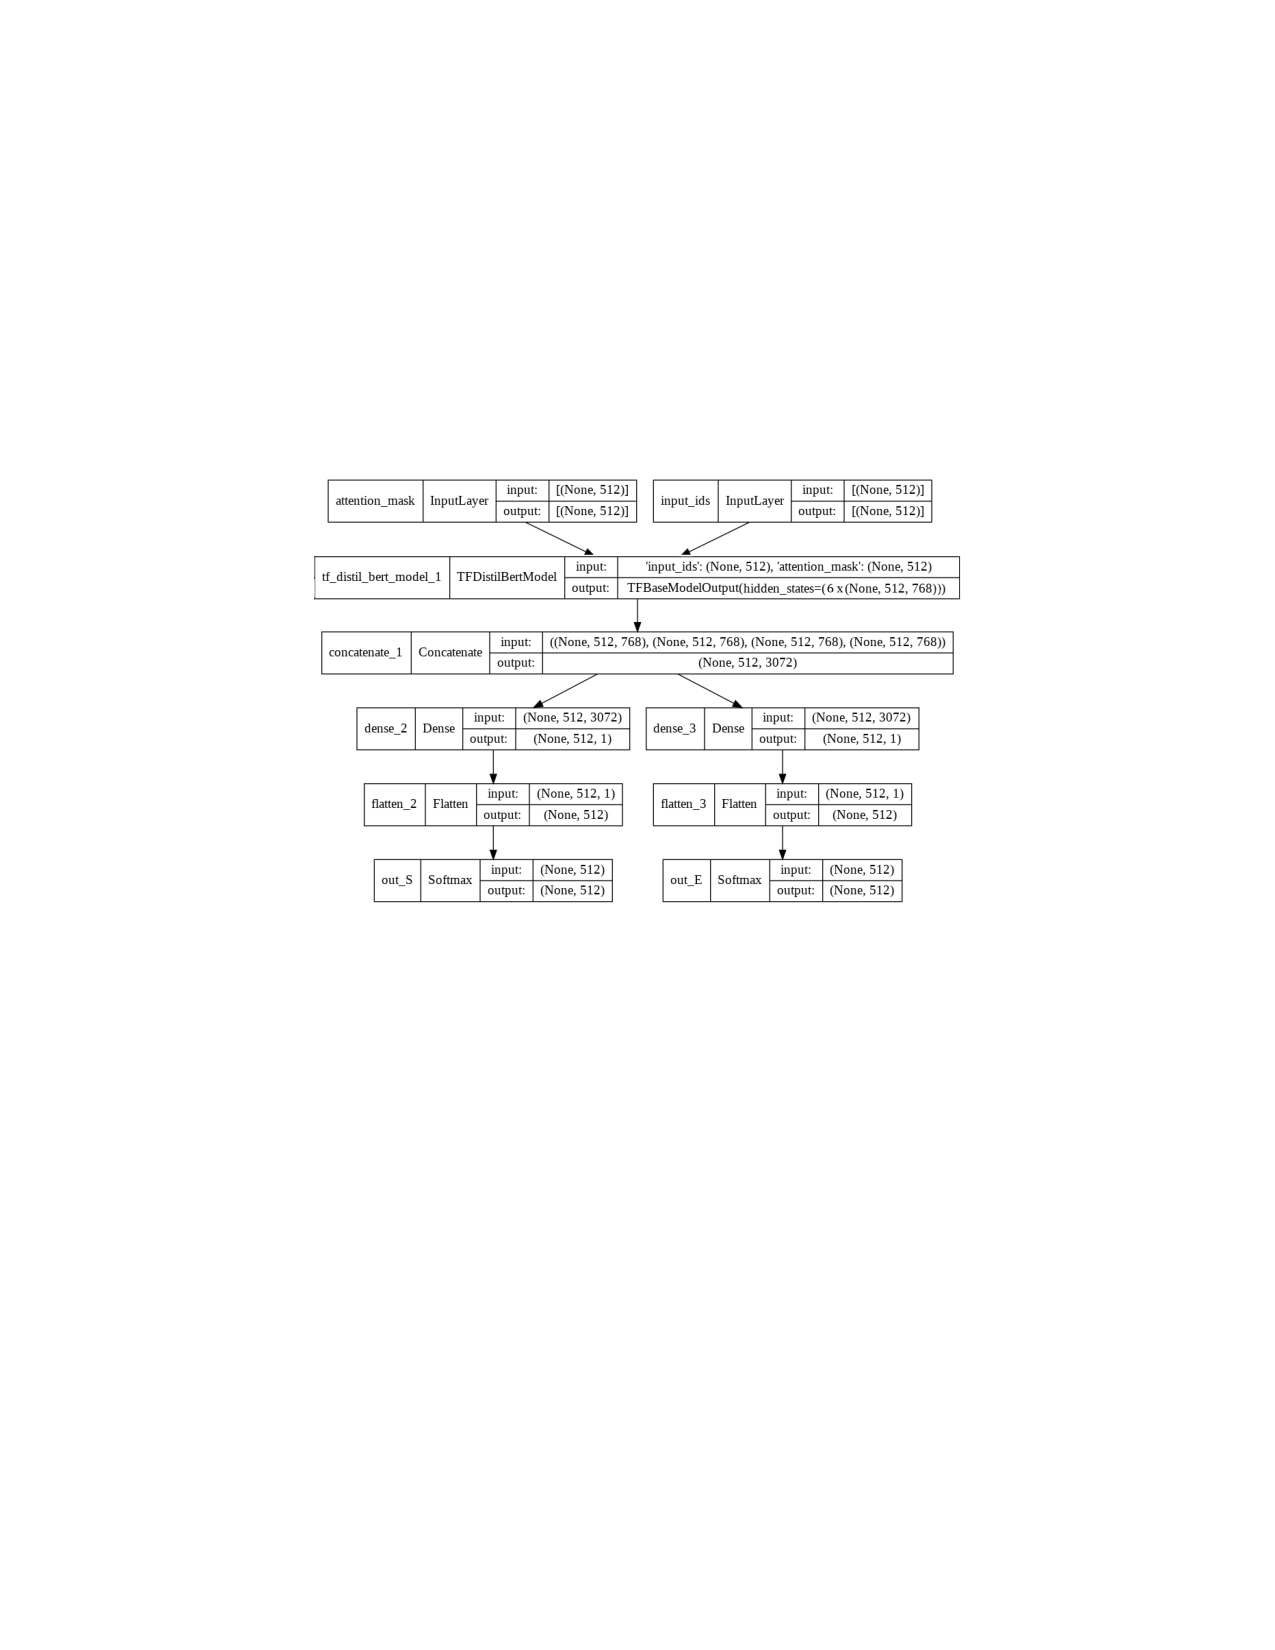
\includegraphics[width=\textwidth]{img/architecture.pdf}
    \caption{Model architecture}
    \label{fig:architecture}
\end{figure*}
}

The system runs entirely on Python. The dataset is downloaded, denormalized, saved into a DataFrame and extended with the \textit{history} column, which for each dialogue contains a concatenation of the previous dialogues of the same passage, maintaining the original order.

To tackle the Question-Answering task, since the answers should be generated, we implemented a Seq2Seq encoder-decoder model. The EncoderDecoderModel is initialized from a pretrained encoder checkpoint and a pretrained decoder checkpoint. Both the encoder and decoder part are initialized from an encoder-only model checkpoint, chosen between BERT-Tiny or DistilRoBERTa, \textbf{both contained in the HuggingFace library}. Before passing the input data to the model, the data is encoded by using a pretrained tokenizer, that is instantiated by the AutoTokenizer class of the HuggingFace library. The tokenizer is used to concatenate and to encode question(, history) and context strings into single arrays of tokens, which are then used to feed the encoder, and instead the answer strings are encoded separately and passed as input to the decoder. The answers are generated by leveraging as decoding strategy the beam search technique.

The models are implemented and trained using the Pytorch framework for reproducibility and experimental reasons. In particular the Pytorch Dataset is built using the input encodings returned from the tokenizer, and then the Pytorch Dataloader is used to wrap an iterable around the Dataset to easily retrieve the data during the training process.

%For the model architectures, see Figure~\ref{fig:model_architecture}.

\begin{table*}[!t]
\centering
\begin{tabular}{l|l|l|c|c|c}
\multicolumn{1}{c|}{\textbf{Model}} & \textbf{History} & \textbf{Seed} & \textbf{Validation loss} & \textbf{Validation F1} & \textbf{Test F1} \\ \hline
BERT-Tiny   & no    & 42    & 3.555		& 16.582   & 17.571\\
BERT-Tiny   & no    & 2022    & 3.550	& 16.650	& 17.162\\
BERT-Tiny   & no    & 1377    & 3.559	& 16.330	& 17.013\\
BERT-Tiny   & yes    & 42    & 3.569	& 15.726	& 16.4511\\
BERT-Tiny   & yes    & 2022    & 3.553	& 15.927	& 16.819\\
BERT-Tiny   & yes    & 1377    & 3.555	& 15.549	& 16.160\\
DistilRoBERTa   & no    & 42    & 1.825	& 48.576	& 50.074\\
DistilRoBERTa   & no    & 2022    & 1.880	& 48.715	& 50.355\\
DistilRoBERTa   & no    & 1377    & 1.871	& 47.900	& 50.250\\
DistilRoBERTa   & yes    & 42    & 1.565	& 56.382	& 58.433\\
DistilRoBERTa   & yes    & 2022    & 1.601	& 56.206	& 58.676\\
DistilRoBERTa   & yes    & 1377    & 1.582	& 54.847	& 57.102\\
\end{tabular}
\caption{Results obtained with all the possible configurations for the two models}
\label{table:1}
\end{table*}

\section{Experimental setup and results}
\label{sec:results}
\attention{MAX 1 COLUMN FOR ASSIGNMENT REPORTS / 3 COLUMNS FOR PROJECT OR PW / 5 FOR COMBINED REPORTS.}

\explanation{
Describe how you set up your experiments: which architectures/configurations you used, which hyper-parameters and what methods used to set them, which optimizers, metrics, etc.
\\
Then, \textbf{use tables} to summarize your your findings (numerical results) in validation and test. If you don't have experience with tables in \LaTeX, you might want to use \href{https://www.tablesgenerator.com/}{\LaTeX table generator} to quickly create a table template.
}

Both the pretrained models were fine-tuned with different configurations of \textit{seed} and \textit{dialogue history usage}, in a totally reproducible way.
The split of the Dataset was the same for every run, and the dataset's rows were randomly shuffled to avoid getting stuck in a local minima. The encoding length used was the maximum supported by the models, while the max length of the decoder was of 64 tokens.
The optimizer used for training is AdamW, and the allennlp implementation of the SQUAD-F1 score was used as evaluation's metric. 
After some tests it was clear that to have the best performance on BERT-Tiny and DistilRoBERTa the learning rate was model dependent (respectively of \num{4e-4} and \num{4e-5}). The fine-tuning phase used the whole training set and lasted 3 epochs for each model, using a \textit{batch size} of 16. The sections \textit{Define Model} and \textit{Training} contain the variables that are used to set the hyperparameters to produce a specific model, these variables were changed at each run.
The evaluation's results are described in Table \ref{table:1}.

\section{Discussion}
\label{sec:discussion}
\attention{MAX 1.5 COLUMNS FOR ASSIGNMENT REPORTS / 3 COLUMNS FOR PROJECT / 4 FOR COMBINED REPORTS. ADDITIONAL EXAMPLES COULD BE PLACED IN AN APPENDIX AFTER THE REFERENCES IF THEY DO NOT FIT HERE.}


\explanation{
Here you should make your analysis of the results you obtained in your experiments. Your discussion should be structured in two parts: 
\begin{itemize}
    \item discussion of quantitative results (based on the metrics you have identified earlier; compare with baselines);
    \item error analysis: show some examples of odd/wrong/unwanted  outputs; reason about why you are getting those results, elaborate on what could/should be changed in future developments of this work.
\end{itemize}
}

The difference between different seeds of the same model is negligible (always under 1\% except for DistilRoBERTa with history).

The performance difference between the two models is striking: BERT-Tiny reached a disappointing maximum F1 score on the test set of 17.6 while DistilRoBERTa-base reached an acceptable 58.7. This explainable by the difference in complexity of the models (4.4M vs 82M parameters) \cite{turc2019wellread}\cite{sanh2020distilbert}.

BERT-Tiny performed sightly better without history while DistilRoBERTa-base performed much better with the history. DistilRoBERTa's behavior was the expected one, a possible culprit for BERT-Tiny strange behavior and overall poor performance could be the inability to handle the added lexycal and semantical complexity added by the history.

We analyzed the errors made by all models on various types of question and the results are visible in Figure~\ref{fig:wrong_1} and Figure~\ref{fig:wrong_2}. Besides confirming the observations made above, we can observe that the most difficult questions are those requiring the history and those with the least distribution.

We realized a truncation analysis of every model which showed that inputs truncated because of the limited encoding length accounted only for 3\% of the errors. This means that even with a sliding window approach there wouldn't be much difference in the number of errors.

\section{Conclusion}
\label{sec:conclusion}
\attention{MAX 1 COLUMN.}

\explanation{
In one or two paragraphs, recap your work and main results.
What did you observe? 
Did all go according to expectations? 
Was there anything surprising or worthwhile mentioning?
After that, discuss the main limitations of the solution you have implemented, and indicate promising directions for future improvement.
}

This problem relies heavily on identifying the semantic meaning of questions and answers and existing literature highlights the importance of model size on this kind of task, so an obvious but costly way to improve the output would be to increase the size of the model \cite{wei2022emergent}. A less naive way to improve the performance would be to use a pre-trained question answering model instead of a generic model.

\section{Links to external resources}
\label{sec:links}
\attention{THIS SECTION IS OPTIONAL}
\explanation{
Insert here:
\begin{itemize}
    \item a link to your GitHub or any other public repo where one can find your code (only if you did not submit your code on Virtuale); 
    \item a link to your dataset (only for non-standard projects or project works).
\end{itemize}
}
\begin{itemize}[noitemsep,nolistsep]
    \item \href{https://stanfordnlp.github.io/coqa/}{CoQa Dataset} \cite{https://doi.org/10.48550/arxiv.1808.07042}
    \item \href{https://github.com/Danysan1/ai-unibo-nlp-project}{Our GitHub repository}
\end{itemize}

\attention{DO NOT INSERT CODE IN THIS REPORT}
%\bibliography{nlpreport.bib}

\bibliography{nlpreport, main}

\appendix
\section{Appendix}

\begin{figure*}
    \centering
    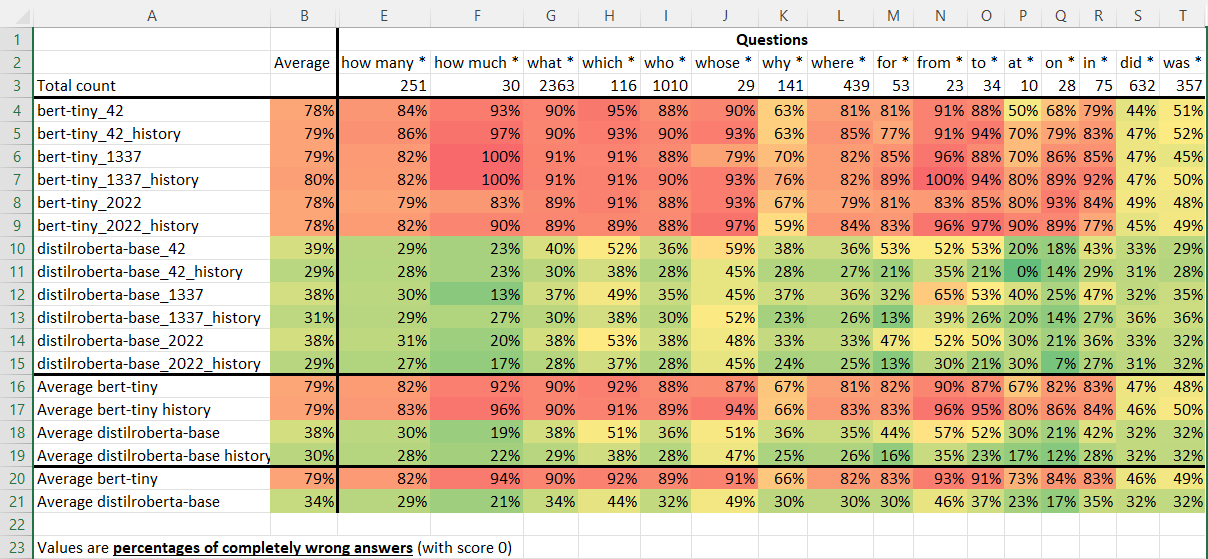
\includegraphics[width=\textwidth]{img/worst_results_1.png}
    \caption{Test results: percentages of wrong answers by question type}
    \label{fig:wrong_1}
\end{figure*}

\begin{figure*}
    \centering
    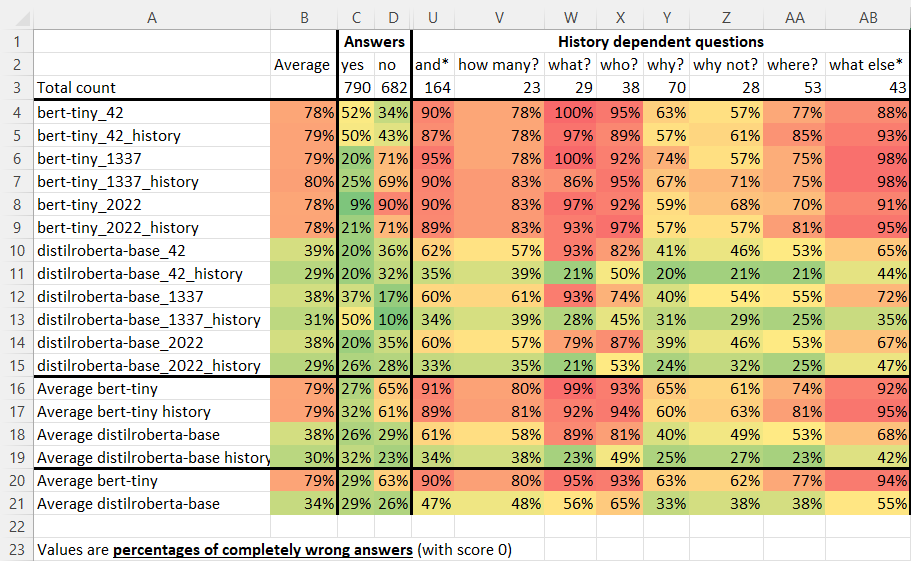
\includegraphics[width=\textwidth]{img/worst_results_2.png}
    \caption{Test results: percentages of wrong answers by answer or by history-dependent question type}
    \label{fig:wrong_2}
\end{figure*}

\end{document}